\documentclass[a4paper]{acm_proc_article-sp}  
\usepackage{microtype}
\usepackage{mathpazo}
\usepackage{listings}
\usepackage{xspace}
\usepackage{array}
\usepackage{tikz}
\newcommand{\eg}{e.g.\@\xspace}
\newcommand{\ie}{i.e.\@\xspace}
\newcommand{\etc}{etc.\@\xspace}
\newcommand{\Naive}{Na\"{i}ve\@\xspace}
\newcommand{\naive}{na\"{i}ve\@\xspace}
\lstset{language=python}
\begin{document}

\title{The Mitar Method of Ultimate Fairness}
\author{\alignauthor Mitar Milutinovi\'{c} and Valkyrie Savage\\
\affaddr{Computer Science Division\\University of California, Berkeley} \\
\email{mitar@tnode.net valkyrie@eecs.berkeley.edu}\\
\text{CS270 Final Project, Spring 2013}
} 
\maketitle

\setcounter{page}{1}
\pagenumbering{arabic}

\section{Abstract}

We designed a voting schema which allows a group of people to better decide on a common opinion about an issue. Currently,
the most used approach is to simply count number of votes against and for, while not taking into account people who do
not cast a vote. Our approach is to have each person define delegates whose votes will be counted when he/she does not
vote him/herself. In this way we get a social network, a trust network, between users which can be
used to transitively compute missing votes. We believe such a result better represents the will of the group.

\section{Introduction}

Something will go here.

\section{Related Work}

\begin{tabular}{p{1.75cm} || p{1.75cm} | p{1.75cm} | p{1.75cm} | p{1.75cm} | p{1.75cm} | p{1.75cm} | p{1.75cm}}
   & Helios & Liquid Feedback & Schulze Method & Yamakawa, et al. & Smartocracy & Anderson, et al. & MM \\
  \hline \hline
  delegation & no & yes & no & yes & yes & ande & yes \\
  \hline
  ranking & no & no & yes & no & no & ande & no \\
  \hline
  runtime & helios & lf & sm & y & sma & ande & mm \\
  \hline
  satisfactory result & helios & lf & sm & y & sma & ande & mm \\
  \hline
  secure & yes & yes? & depends & no & yes & ande & yes \\
  \hline
  secret & yes & no & depends & no & yes & ande & yes \\
  \hline
  illustration & 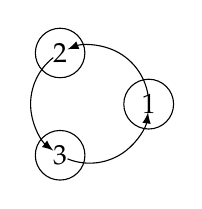
\begin{tikzpicture}

\def \n {3}
\def \radius {.75cm}
\def \margin {8} % margin in angles, depends on the radius

\foreach \s in {1,...,\n}
{
  \node[draw, circle] at ({360/\n * (\s - 1)}:\radius) {$\s$};
  \draw[->, >=latex] ({360/\n * (\s - 1)+\margin}:\radius) 
    arc ({360/\n * (\s - 1)+\margin}:{360/\n * (\s)-\margin}:\radius);
}
\end{tikzpicture}
 & lf & sm & y & sma & ande & mm \\
  \hline
\end{tabular}

\bibliographystyle{abbrv}
\bibliography{mm}
\end{document}
